

% Gradient Info

\tikzset {_9gzeye8sn/.code = {\pgfsetadditionalshadetransform{ \pgftransformshift{\pgfpoint{0 bp } { 0 bp }  }  \pgftransformrotate{0 }  \pgftransformscale{2 }  }}}
\pgfdeclarehorizontalshading{_p4qtkslv0}{150bp}{rgb(0bp)=(0.96,0.65,0.14);
rgb(37.5bp)=(0.96,0.65,0.14);
rgb(37.5bp)=(0.96,0.65,0.14);
rgb(62.5bp)=(0.72,0.91,0.53);
rgb(100bp)=(0.72,0.91,0.53)}

% Gradient Info

\tikzset {_fkkmn7hul/.code = {\pgfsetadditionalshadetransform{ \pgftransformshift{\pgfpoint{0 bp } { 0 bp }  }  \pgftransformrotate{0 }  \pgftransformscale{2 }  }}}
\pgfdeclarehorizontalshading{_2a3my88uk}{150bp}{rgb(0bp)=(0.96,0.65,0.14);
rgb(37.5bp)=(0.96,0.65,0.14);
rgb(62.5bp)=(0.72,0.91,0.53);
rgb(100bp)=(0.72,0.91,0.53)}
\tikzset{every picture/.style={line width=0.75pt}} %set default line width to 0.75pt

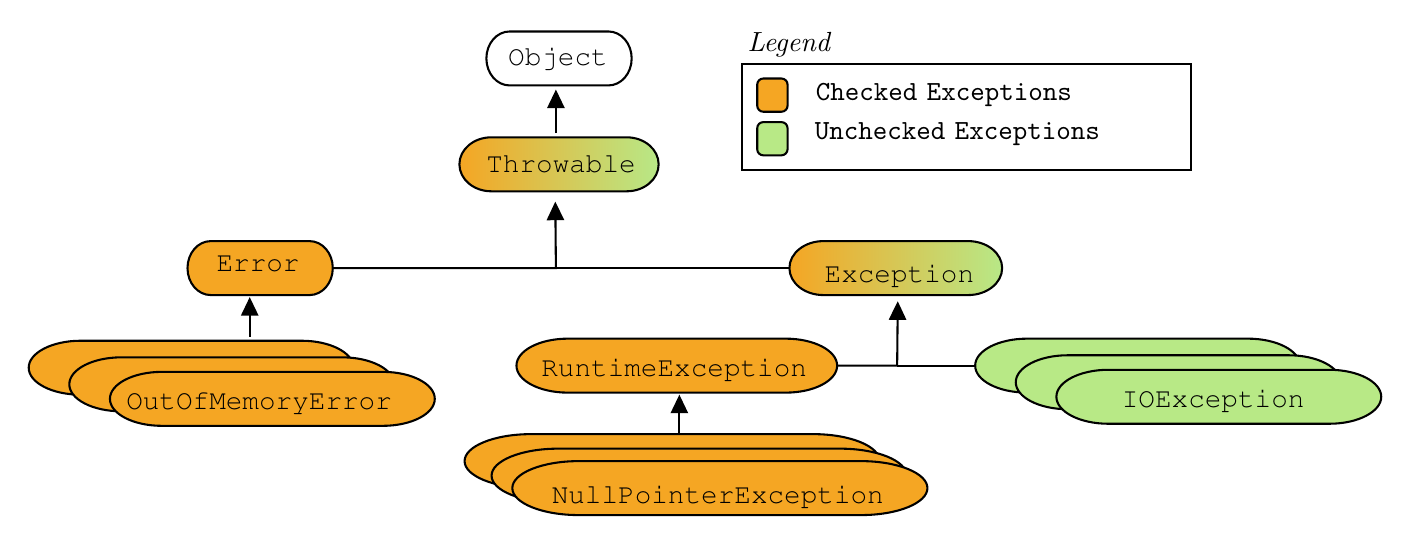
\begin{tikzpicture}[x=0.75pt,y=0.75pt,yscale=-1,xscale=1]
%uncomment if require: \path (0,443); %set diagram left start at 0, and has height of 443

%Flowchart: Terminator [id:dp6117160387653431]
\draw   (408.2,28) -- (455.8,28) .. controls (461.99,28) and (467,33.82) .. (467,41) .. controls (467,48.18) and (461.99,54) .. (455.8,54) -- (408.2,54) .. controls (402.01,54) and (397,48.18) .. (397,41) .. controls (397,33.82) and (402.01,28) .. (408.2,28) -- cycle ;
%Flowchart: Terminator [id:dp010853834463749212]
\path  [shading=_p4qtkslv0,_9gzeye8sn] (399.36,79) -- (464.64,79) .. controls (473.12,79) and (480,84.82) .. (480,92) .. controls (480,99.18) and (473.12,105) .. (464.64,105) -- (399.36,105) .. controls (390.88,105) and (384,99.18) .. (384,92) .. controls (384,84.82) and (390.88,79) .. (399.36,79) -- cycle ; % for fading
 \draw   (399.36,79) -- (464.64,79) .. controls (473.12,79) and (480,84.82) .. (480,92) .. controls (480,99.18) and (473.12,105) .. (464.64,105) -- (399.36,105) .. controls (390.88,105) and (384,99.18) .. (384,92) .. controls (384,84.82) and (390.88,79) .. (399.36,79) -- cycle ; % for border

%Flowchart: Terminator [id:dp157767405099974]
\draw  [fill={rgb, 255:red, 245; green, 166; blue, 35 }  ,fill opacity=1 ] (264.2,129) -- (311.8,129) .. controls (317.99,129) and (323,134.82) .. (323,142) .. controls (323,149.18) and (317.99,155) .. (311.8,155) -- (264.2,155) .. controls (258.01,155) and (253,149.18) .. (253,142) .. controls (253,134.82) and (258.01,129) .. (264.2,129) -- cycle ;
%Flowchart: Terminator [id:dp5141793073831367]
\path  [shading=_2a3my88uk,_fkkmn7hul] (559.4,129) -- (629.1,129) .. controls (638.16,129) and (645.5,134.82) .. (645.5,142) .. controls (645.5,149.18) and (638.16,155) .. (629.1,155) -- (559.4,155) .. controls (550.34,155) and (543,149.18) .. (543,142) .. controls (543,134.82) and (550.34,129) .. (559.4,129) -- cycle ; % for fading
 \draw   (559.4,129) -- (629.1,129) .. controls (638.16,129) and (645.5,134.82) .. (645.5,142) .. controls (645.5,149.18) and (638.16,155) .. (629.1,155) -- (559.4,155) .. controls (550.34,155) and (543,149.18) .. (543,142) .. controls (543,134.82) and (550.34,129) .. (559.4,129) -- cycle ; % for border

%Flowchart: Terminator [id:dp5847558830238542]
\draw  [fill={rgb, 255:red, 245; green, 166; blue, 35 }  ,fill opacity=1 ] (436.22,176) -- (541.28,176) .. controls (554.93,176) and (566,181.82) .. (566,189) .. controls (566,196.18) and (554.93,202) .. (541.28,202) -- (436.22,202) .. controls (422.57,202) and (411.5,196.18) .. (411.5,189) .. controls (411.5,181.82) and (422.57,176) .. (436.22,176) -- cycle ;
%Flowchart: Terminator [id:dp09560156756174476]
\draw  [fill={rgb, 255:red, 245; green, 166; blue, 35 }  ,fill opacity=1 ] (418.5,222) -- (554.5,222) .. controls (572.17,222) and (586.5,227.82) .. (586.5,235) .. controls (586.5,242.18) and (572.17,248) .. (554.5,248) -- (418.5,248) .. controls (400.83,248) and (386.5,242.18) .. (386.5,235) .. controls (386.5,227.82) and (400.83,222) .. (418.5,222) -- cycle ;
%Flowchart: Terminator [id:dp1722169871719902]
\draw  [fill={rgb, 255:red, 245; green, 166; blue, 35 }  ,fill opacity=1 ] (201.54,177) -- (307.97,177) .. controls (321.8,177) and (333.01,182.82) .. (333.01,190) .. controls (333.01,197.18) and (321.8,203) .. (307.97,203) -- (201.54,203) .. controls (187.71,203) and (176.5,197.18) .. (176.5,190) .. controls (176.5,182.82) and (187.71,177) .. (201.54,177) -- cycle ;
%Flowchart: Terminator [id:dp06414597564774949]
\draw  [fill={rgb, 255:red, 245; green, 166; blue, 35 }  ,fill opacity=1 ] (221.11,185) -- (327.54,185) .. controls (341.37,185) and (352.58,190.82) .. (352.58,198) .. controls (352.58,205.18) and (341.37,211) .. (327.54,211) -- (221.11,211) .. controls (207.28,211) and (196.06,205.18) .. (196.06,198) .. controls (196.06,190.82) and (207.28,185) .. (221.11,185) -- cycle ;
%Flowchart: Terminator [id:dp5021023318971636]
\draw  [fill={rgb, 255:red, 245; green, 166; blue, 35 }  ,fill opacity=1 ] (240.67,192) -- (347.1,192) .. controls (360.93,192) and (372.14,197.82) .. (372.14,205) .. controls (372.14,212.18) and (360.93,218) .. (347.1,218) -- (240.67,218) .. controls (226.84,218) and (215.63,212.18) .. (215.63,205) .. controls (215.63,197.82) and (226.84,192) .. (240.67,192) -- cycle ;
%Flowchart: Terminator [id:dp9011559544249151]
\draw  [fill={rgb, 255:red, 245; green, 166; blue, 35 }  ,fill opacity=1 ] (431.5,229) -- (567.5,229) .. controls (585.17,229) and (599.5,234.82) .. (599.5,242) .. controls (599.5,249.18) and (585.17,255) .. (567.5,255) -- (431.5,255) .. controls (413.83,255) and (399.5,249.18) .. (399.5,242) .. controls (399.5,234.82) and (413.83,229) .. (431.5,229) -- cycle ;
%Flowchart: Terminator [id:dp09475948376995225]
\draw  [fill={rgb, 255:red, 245; green, 166; blue, 35 }  ,fill opacity=1 ] (441.5,235) -- (577.5,235) .. controls (595.17,235) and (609.5,240.82) .. (609.5,248) .. controls (609.5,255.18) and (595.17,261) .. (577.5,261) -- (441.5,261) .. controls (423.83,261) and (409.5,255.18) .. (409.5,248) .. controls (409.5,240.82) and (423.83,235) .. (441.5,235) -- cycle ;
%Flowchart: Terminator [id:dp8075708913459207]
\draw  [fill={rgb, 255:red, 184; green, 233; blue, 134 }  ,fill opacity=1 ] (657.54,176) -- (763.97,176) .. controls (777.8,176) and (789.01,181.82) .. (789.01,189) .. controls (789.01,196.18) and (777.8,202) .. (763.97,202) -- (657.54,202) .. controls (643.71,202) and (632.5,196.18) .. (632.5,189) .. controls (632.5,181.82) and (643.71,176) .. (657.54,176) -- cycle ;
%Flowchart: Terminator [id:dp8051439840182716]
\draw  [fill={rgb, 255:red, 184; green, 233; blue, 134 }  ,fill opacity=1 ] (677.11,184) -- (783.54,184) .. controls (797.37,184) and (808.58,189.82) .. (808.58,197) .. controls (808.58,204.18) and (797.37,210) .. (783.54,210) -- (677.11,210) .. controls (663.28,210) and (652.06,204.18) .. (652.06,197) .. controls (652.06,189.82) and (663.28,184) .. (677.11,184) -- cycle ;
%Flowchart: Terminator [id:dp13997636092463628]
\draw  [fill={rgb, 255:red, 184; green, 233; blue, 134 }  ,fill opacity=1 ] (696.67,191) -- (803.1,191) .. controls (816.93,191) and (828.14,196.82) .. (828.14,204) .. controls (828.14,211.18) and (816.93,217) .. (803.1,217) -- (696.67,217) .. controls (682.84,217) and (671.63,211.18) .. (671.63,204) .. controls (671.63,196.82) and (682.84,191) .. (696.67,191) -- cycle ;
%Straight Lines [id:da007793310239582185]
\draw    (430.5,77) -- (430.5,59) ;
\draw [shift={(430.5,56)}, rotate = 450] [fill={rgb, 255:red, 0; green, 0; blue, 0 }  ][line width=0.08]  [draw opacity=0] (8.93,-4.29) -- (0,0) -- (8.93,4.29) -- cycle    ;
%Straight Lines [id:da3175144297134308]
\draw    (323,142) -- (430.5,142) -- (430.23,113) ;
\draw [shift={(430.2,110)}, rotate = 449.47] [fill={rgb, 255:red, 0; green, 0; blue, 0 }  ][line width=0.08]  [draw opacity=0] (8.93,-4.29) -- (0,0) -- (8.93,4.29) -- cycle    ;
%Straight Lines [id:da4184906006596295]
\draw    (543,142) -- (430.5,142) ;
%Straight Lines [id:da8165614272716485]
\draw    (282.98,175) -- (282.98,159) ;
\draw [shift={(282.98,156)}, rotate = 450] [fill={rgb, 255:red, 0; green, 0; blue, 0 }  ][line width=0.08]  [draw opacity=0] (8.93,-4.29) -- (0,0) -- (8.93,4.29) -- cycle    ;
%Straight Lines [id:da9159581853872254]
\draw    (489.98,222) -- (489.98,206) ;
\draw [shift={(489.98,203)}, rotate = 450] [fill={rgb, 255:red, 0; green, 0; blue, 0 }  ][line width=0.08]  [draw opacity=0] (8.93,-4.29) -- (0,0) -- (8.93,4.29) -- cycle    ;
%Straight Lines [id:da7822720632034224]
\draw    (566,189) -- (594.91,189) -- (595.18,161) ;
\draw [shift={(595.2,158)}, rotate = 450.55] [fill={rgb, 255:red, 0; green, 0; blue, 0 }  ][line width=0.08]  [draw opacity=0] (8.93,-4.29) -- (0,0) -- (8.93,4.29) -- cycle    ;
%Straight Lines [id:da43465237471765317]
\draw    (632.5,189) -- (594.91,189) ;
%Shape: Rectangle [id:dp9947647476097804]
\draw   (520,43.67) -- (736.5,43.67) -- (736.5,94.67) -- (520,94.67) -- cycle ;
%Rounded Rect [id:dp9583520358108684]
\draw  [fill={rgb, 255:red, 245; green, 166; blue, 35 }  ,fill opacity=1 ] (527.49,53.59) .. controls (527.49,51.98) and (528.8,50.67) .. (530.41,50.67) -- (539.19,50.67) .. controls (540.8,50.67) and (542.11,51.98) .. (542.11,53.59) -- (542.11,63.74) .. controls (542.11,65.36) and (540.8,66.67) .. (539.19,66.67) -- (530.41,66.67) .. controls (528.8,66.67) and (527.49,65.36) .. (527.49,63.74) -- cycle ;
%Rounded Rect [id:dp12081524058509086]
\draw  [fill={rgb, 255:red, 184; green, 233; blue, 134 }  ,fill opacity=1 ] (527.49,74.59) .. controls (527.49,72.98) and (528.8,71.67) .. (530.41,71.67) -- (539.19,71.67) .. controls (540.8,71.67) and (542.11,72.98) .. (542.11,74.59) -- (542.11,84.74) .. controls (542.11,86.36) and (540.8,87.67) .. (539.19,87.67) -- (530.41,87.67) .. controls (528.8,87.67) and (527.49,86.36) .. (527.49,84.74) -- cycle ;

% Text Node
\draw (406,34) node [anchor=north west][inner sep=0.75pt]   [align=left] {{\fontfamily{pcr}\selectfont Object}};
% Text Node
\draw (395.5,86) node [anchor=north west][inner sep=0.75pt]   [align=left] {{\fontfamily{pcr}\selectfont Throwable}};
% Text Node
\draw (265.5,134.5) node [anchor=north west][inner sep=0.75pt]  [color={rgb, 255:red, 0; green, 0; blue, 0 }  ,opacity=1 ] [align=left] {{\fontfamily{pcr}\selectfont Error}};
% Text Node
\draw (558.5,138.5) node [anchor=north west][inner sep=0.75pt]  [color={rgb, 255:red, 0; green, 0; blue, 0 }  ,opacity=1 ] [align=left] {{\fontfamily{pcr}\selectfont Exception}};
% Text Node
\draw (422,184) node [anchor=north west][inner sep=0.75pt]  [color={rgb, 255:red, 0; green, 0; blue, 0 }  ,opacity=1 ] [align=left] {{\fontfamily{pcr}\selectfont RuntimeException}};
% Text Node
\draw (427,245) node [anchor=north west][inner sep=0.75pt]  [color={rgb, 255:red, 0; green, 0; blue, 0 }  ,opacity=1 ] [align=left] {{\fontfamily{pcr}\selectfont NullPointerException}};
% Text Node
\draw (222,200) node [anchor=north west][inner sep=0.75pt]  [color={rgb, 255:red, 0; green, 0; blue, 0 }  ,opacity=1 ] [align=left] {{\fontfamily{pcr}\selectfont OutOfMemoryError}};
% Text Node
\draw (701.67,199) node [anchor=north west][inner sep=0.75pt]  [color={rgb, 255:red, 0; green, 0; blue, 0 }  ,opacity=1 ] [align=left] {{\fontfamily{pcr}\selectfont \textcolor[rgb]{0,0,0}{IOException}}};
% Text Node
\draw (554.23,51.4) node [anchor=north west][inner sep=0.75pt]    {$\mathtt{Checked\ Exceptions}$};
% Text Node
\draw (553.72,70.4) node [anchor=north west][inner sep=0.75pt]    {$\mathtt{Unchecked\ Exceptions}$};
% Text Node
\draw (521.35,26.67) node [anchor=north west][inner sep=0.75pt]   [align=left] {\textit{Legend}};


\end{tikzpicture}
